% Figure: Whole-Body ME/CFS Systems Model Architecture
% Shows 7 subsystem modules in circular layout with labeled coupling arrows

\begin{figure}[htbp]
\centering
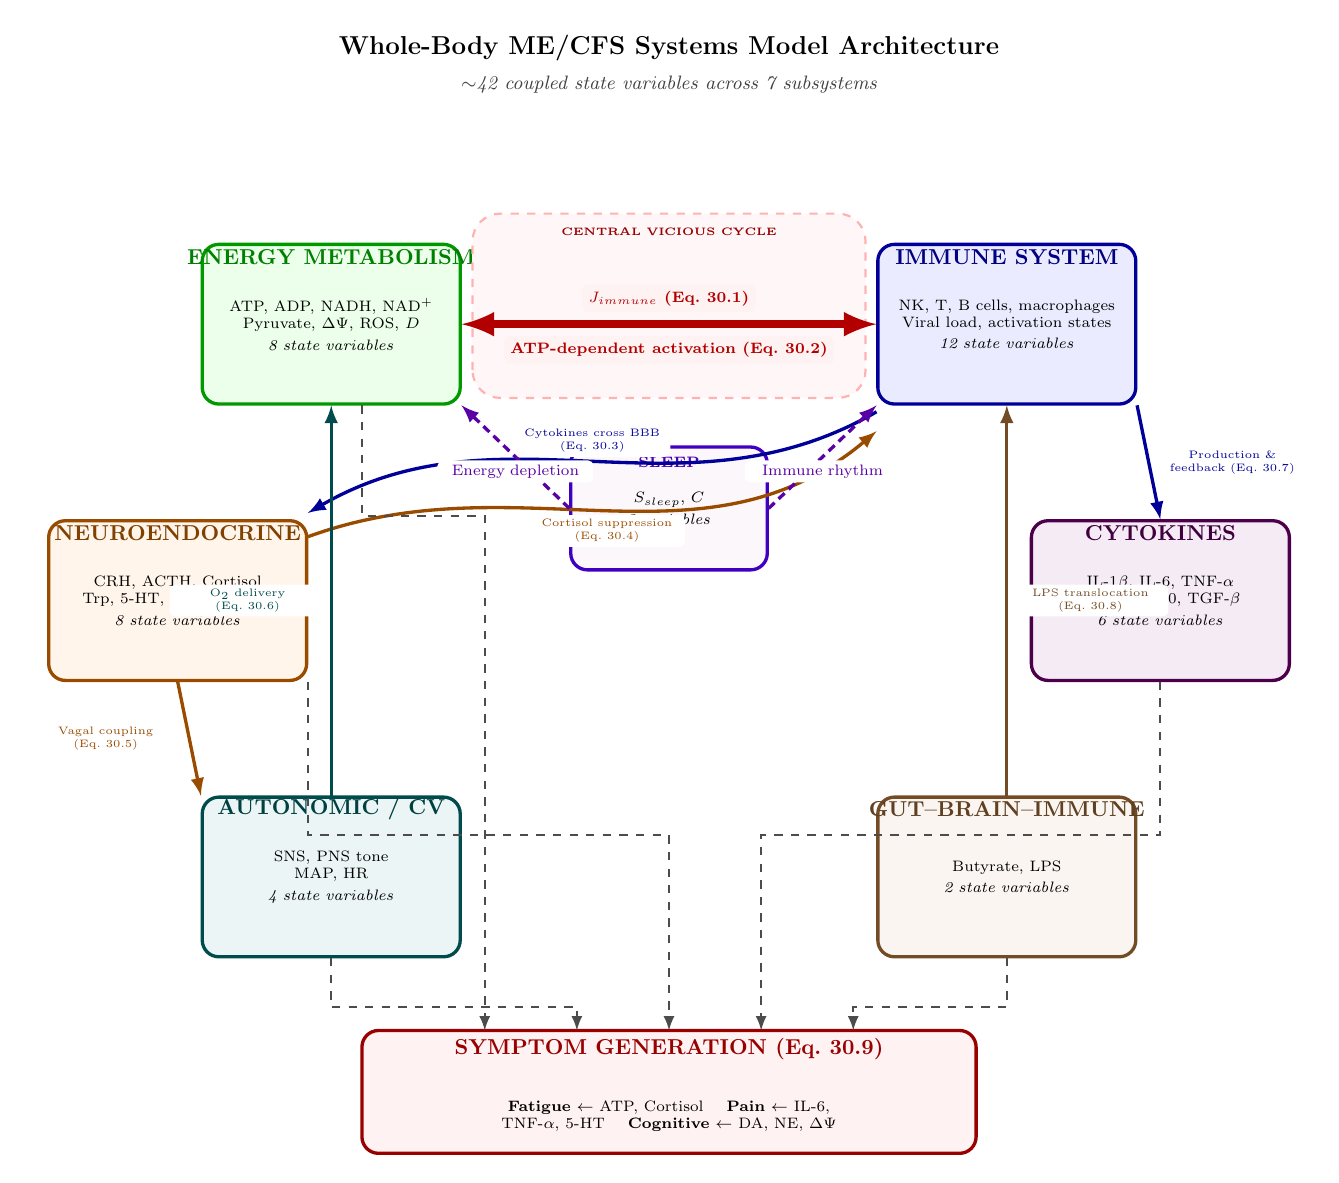
\begin{tikzpicture}[
    scale=0.78, every node/.style={scale=0.78},
    % Subsystem box styles
    subsystem/.style={draw=black!70, very thick, rounded corners=6pt,
        minimum width=4.2cm, minimum height=2.6cm, align=center, inner sep=5pt},
    energy-sys/.style={subsystem, draw=green!60!black, fill=green!8},
    immune-sys/.style={subsystem, draw=blue!60!black, fill=blue!8},
    cytokine-sys/.style={subsystem, draw=violet!60!black, fill=violet!8},
    neuro-sys/.style={subsystem, draw=orange!60!black, fill=orange!8},
    auto-sys/.style={subsystem, draw=teal!60!black, fill=teal!8},
    gut-sys/.style={subsystem, draw=brown!60!black, fill=brown!8},
    sleep-sys/.style={subsystem, draw=blue!50!violet, fill=blue!3!violet!3,
        minimum width=3.2cm, minimum height=2cm},
    symptom-sys/.style={draw=red!60!black, fill=red!5, very thick,
        rounded corners=6pt, minimum width=10cm, minimum height=2cm,
        align=center, inner sep=5pt},
    % Arrow styles
    coupling/.style={-latex, thick, line width=1.2pt},
    vicious/.style={latex-latex, ultra thick, red!70!black, line width=3pt},
    symptom-arrow/.style={-latex, thick, dashed, gray!60!black},
    % Label styles
    mechanism/.style={font=\tiny, fill=white, inner sep=2pt, rounded corners=2pt,
        text width=2.4cm, align=center},
]

% === TITLE ===
\node[font=\large\bfseries] at (0, 10.5) {Whole-Body ME/CFS Systems Model Architecture};
\node[font=\small\itshape, gray!50!black] at (0, 9.9) {$\sim$42 coupled state variables across 7 subsystems};

% === SUBSYSTEM NODES (circular layout) ===
% Energy Metabolism (top-left)
\node[energy-sys] (energy) at (-5.5, 6) {};
\node[font=\bfseries, green!50!black] at (-5.5, 7.1) {ENERGY METABOLISM};
\node[font=\scriptsize, text width=3.8cm, align=center] at (-5.5, 6) {
    ATP, ADP, NADH, NAD\textsuperscript{+}\\
    Pyruvate, $\Delta\Psi$, ROS, $D$\\[2pt]
    \textit{8 state variables}
};

% Immune System (top-right)
\node[immune-sys] (immune) at (5.5, 6) {};
\node[font=\bfseries, blue!50!black] at (5.5, 7.1) {IMMUNE SYSTEM};
\node[font=\scriptsize, text width=3.8cm, align=center] at (5.5, 6) {
    NK, T, B cells, macrophages\\
    Viral load, activation states\\[2pt]
    \textit{12 state variables}
};

% Cytokines (right)
\node[cytokine-sys] (cytokine) at (8, 1.5) {};
\node[font=\bfseries, violet!50!black] at (8, 2.6) {CYTOKINES};
\node[font=\scriptsize, text width=3.8cm, align=center] at (8, 1.5) {
    IL-1$\beta$, IL-6, TNF-$\alpha$\\
    IFN-$\gamma$, IL-10, TGF-$\beta$\\[2pt]
    \textit{6 state variables}
};

% Neuroendocrine (left)
\node[neuro-sys] (neuro) at (-8, 1.5) {};
\node[font=\bfseries, orange!50!black] at (-8, 2.6) {NEUROENDOCRINE};
\node[font=\scriptsize, text width=3.8cm, align=center] at (-8, 1.5) {
    CRH, ACTH, Cortisol\\
    Trp, 5-HT, Kyn, DA, NE\\[2pt]
    \textit{8 state variables}
};

% Autonomic/Cardiovascular (bottom-left)
\node[auto-sys] (auto) at (-5.5, -3) {};
\node[font=\bfseries, teal!50!black] at (-5.5, -1.9) {AUTONOMIC / CV};
\node[font=\scriptsize, text width=3.8cm, align=center] at (-5.5, -3) {
    SNS, PNS tone\\
    MAP, HR\\[2pt]
    \textit{4 state variables}
};

% Gut-Brain-Immune (bottom-right)
\node[gut-sys] (gut) at (5.5, -3) {};
\node[font=\bfseries, brown!50!black] at (5.5, -1.9) {GUT--BRAIN--IMMUNE};
\node[font=\scriptsize, text width=3.8cm, align=center] at (5.5, -3) {
    Butyrate, LPS\\[2pt]
    \textit{2 state variables}
};

% Sleep (small, upper center)
\node[sleep-sys] (sleep) at (0, 3) {};
\node[font=\bfseries\scriptsize, blue!40!violet] at (0, 3.75) {SLEEP};
\node[font=\scriptsize, text width=2.8cm, align=center] at (0, 3) {
    $S_{\text{sleep}}$, $C$\\[2pt]
    \textit{2 variables}
};

% === CENTRAL VICIOUS CYCLE (Energy <-> Immune) ===
% Highlight box
\draw[red!30, fill=red!3, rounded corners=10pt, dashed, thick]
    (-3.2, 4.8) rectangle (3.2, 7.8);
\node[font=\tiny\bfseries, red!60!black] at (0, 7.5) {CENTRAL VICIOUS CYCLE};

% Bidirectional red arrows
\draw[vicious] (energy.east) -- (immune.west)
    node[midway, above=4pt, font=\scriptsize\bfseries, red!70!black, fill=red!5,
        rounded corners=2pt, inner sep=3pt] {$J_{\text{immune}}$ (Eq.~30.1)}
    node[midway, below=4pt, font=\scriptsize\bfseries, red!70!black, fill=red!5,
        rounded corners=2pt, inner sep=3pt] {ATP-dependent activation (Eq.~30.2)};

% === COUPLING ARROWS ===

% Immune -> Neuroendocrine (cytokines cross BBB)
% Route: from immune south-west corner, curving down to neuro north-east corner
\draw[coupling, blue!60!black]
    ([yshift=-3pt]immune.south west) to[out=210, in=30]
    node[mechanism, pos=0.5, above=2pt] {Cytokines cross BBB\\(Eq.~30.3)}
    ([yshift=3pt]neuro.north east);

% Neuroendocrine -> Immune (cortisol suppression)
% Route: from neuro north-east, curving up to immune south-west — offset to avoid overlap
\draw[coupling, orange!60!black]
    ([yshift=-8pt]neuro.north east) to[out=20, in=220]
    node[mechanism, pos=0.5, below=2pt] {Cortisol suppression\\(Eq.~30.4)}
    ([yshift=-12pt]immune.south west);

% Neuroendocrine -> Autonomic (vagal coupling)
\draw[coupling, orange!60!black] (neuro.south) -- (auto.north west)
    node[mechanism, pos=0.5, left=2pt] {Vagal coupling\\(Eq.~30.5)};

% Autonomic -> Energy (O2 delivery)
\draw[coupling, teal!60!black] (auto.north) -- (energy.south)
    node[mechanism, pos=0.5, left=2pt] {O\textsubscript{2} delivery\\(Eq.~30.6)};

% Immune <-> Cytokines (production and feedback)
\draw[coupling, blue!60!black] (immune.south east) -- (cytokine.north)
    node[mechanism, pos=0.5, right=2pt] {Production \&\\feedback (Eq.~30.7)};

% Gut -> Immune (LPS translocation)
\draw[coupling, brown!60!black] (gut.north) -- (immune.south)
    node[mechanism, pos=0.5, right=2pt] {LPS translocation\\(Eq.~30.8)};

% Sleep connections (lighter)
\draw[coupling, blue!30!violet, densely dashed] (sleep.west) -- (energy.south east)
    node[mechanism, pos=0.5, below=1pt] {\scriptsize Energy depletion};
\draw[coupling, blue!30!violet, densely dashed] (sleep.east) -- (immune.south west)
    node[mechanism, pos=0.5, below=1pt] {\scriptsize Immune rhythm};

% === SYMPTOM GENERATION MODULE (bottom) ===
\node[symptom-sys] (symptoms) at (0, -6.5) {};
\node[font=\bfseries, red!60!black] at (0, -5.8) {SYMPTOM GENERATION (Eq.~30.9)};
\node[font=\scriptsize, text width=9cm, align=center] at (0, -6.9) {
    \textbf{Fatigue} $\leftarrow$ ATP, Cortisol \quad
    \textbf{Pain} $\leftarrow$ IL-6, TNF-$\alpha$, 5-HT \quad
    \textbf{Cognitive} $\leftarrow$ DA, NE, $\Delta\Psi$
};

% Symptom input arrows
\draw[symptom-arrow] (energy.south) ++(0.5,0) -- ++(0,-1.8) -| (-3, -5.5);
\draw[symptom-arrow] (auto.south) -- ++(0,-0.8) -| (-1.5, -5.5);
\draw[symptom-arrow] (neuro.south east) -- ++(0,-2.5) -| (0, -5.5);
\draw[symptom-arrow] (cytokine.south) -- ++(0,-2.5) -| (1.5, -5.5);
\draw[symptom-arrow] (gut.south) -- ++(0,-0.8) -| (3, -5.5);

\end{tikzpicture}
\caption{Architecture of the integrated whole-body model showing subsystem modules
and their couplings. The central energy--immune vicious cycle (red) drives disease
persistence. Arrows indicate the dominant coupling direction; most interactions are
bidirectional. The symptom generation module (bottom) maps physiological states to
clinical symptoms.}
\label{fig:integrated-systems-architecture}
\end{figure}
